\subsubsection{Дисперсионная схема дифракции}
  Дисперсия возникает когда есть некое спектральное распределение источника и
   угол Брегга монохроматора отличается от угла Брегга исследуемого кристалла-образца
   (рисунок \ref{fig:double_crystal_schem_disp_a}).
   коэффициентом отражения.
  \begin{figure}[H]
    \centering
    \subfloat[$\theta_B^M \neq \theta_B^S$]{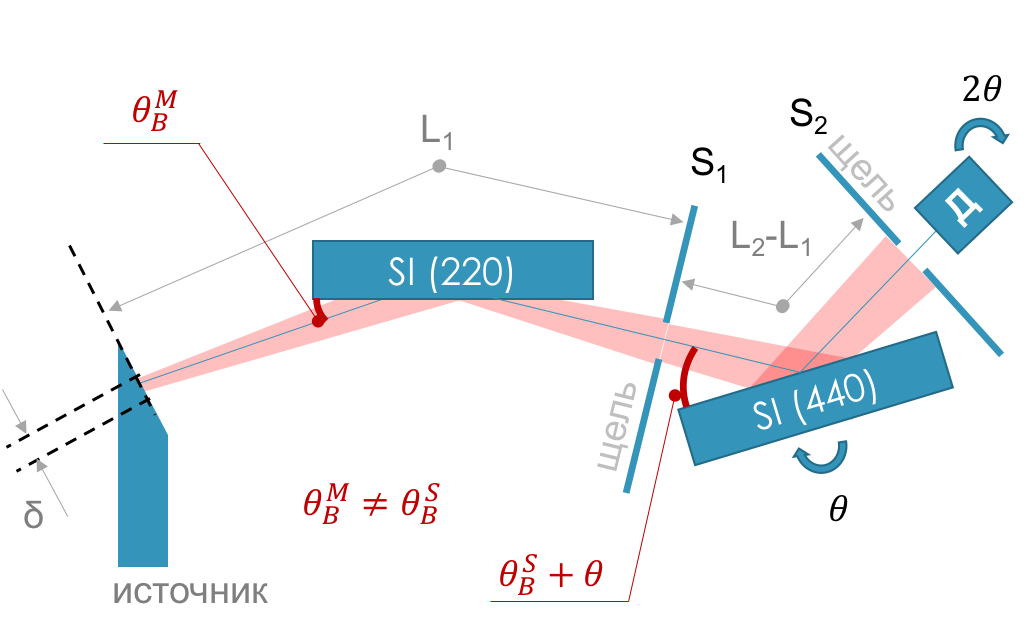
\includegraphics[width=0.6\textwidth]{images/double_crystal_schem_disp.png}\label{fig:double_crystal_schem_disp_a}}
    \hfill
    \subfloat[Спектральное-угловое распределение]{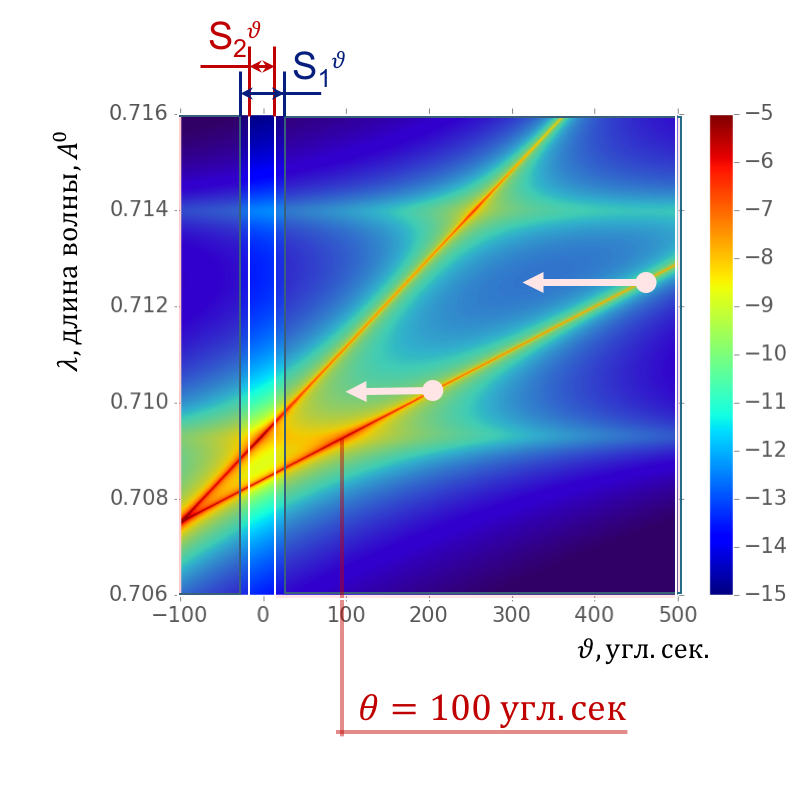
\includegraphics[width=0.35\textwidth]{images/double_crystal_lamtet_disp.png}\label{fig:double_crystal_schem_disp_b}}
    \caption{Дисперсионная схема дифракции}
    \label{ris:double_crystal_schem_disp}
  \end{figure}
  Факт наличия дисперсии возможно проанализировать на спектрально-угловом распределении
  (рисунок \ref{fig:double_crystal_schem_disp_b}), прямая образца в этом случае не параллельна прямой монохроматора и
  в области близкой к точному брегговскому отражению происходит не наложение одной на другую, как в случае отсутствия дисперсии,
  а пересечение. В точке пересечение коэффициент отражения практически равен единице,
  легко заметить что кривая отражения будет уширенной (рисунок \ref{ris:disspersion_curves_expantheory}).
\begin{figure}[H]
  \centering
  \subfloat[Образец Si(440) - $\theta_B = 21.7^o$, $S_1 = S_2 = 100$ мкм.]{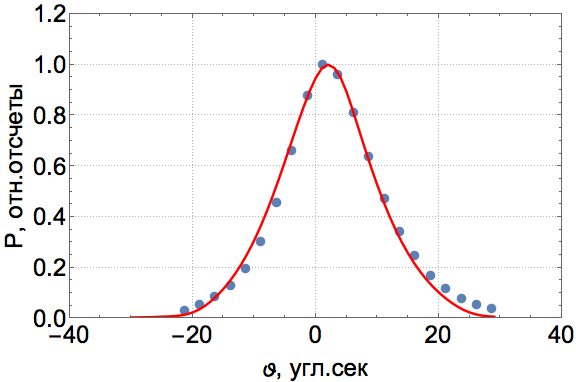
\includegraphics[width=0.45\textwidth]{images/disspers_220_440_100mcm.png}\label{fig:}}
  \hfill
  \subfloat[Образец Si(660) - $\theta_B = 33.7^o$, $S_1 = S_2 = 100$ мкм.]{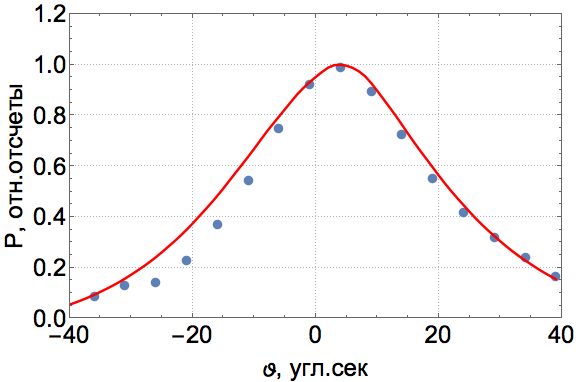
\includegraphics[width=0.45\textwidth]{images/disspers_220_660_100mcm.png}\label{fig:}}
  \hfill
  \subfloat[Образец Si(440) - $\theta_B = 21.7^o$, $S_1 = S_2 = 300$ мкм.]{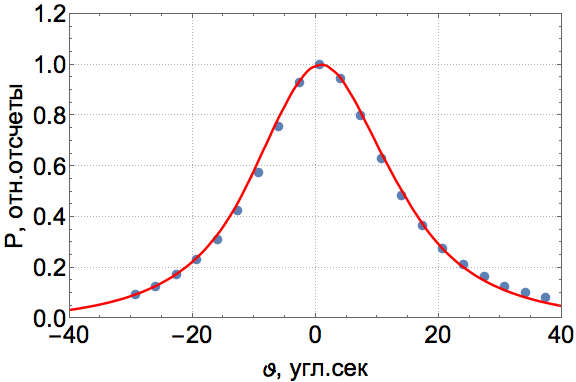
\includegraphics[width=0.45\textwidth]{images/disspers_220_440_300mcm.png}\label{fig:}}
  \hfill
  \subfloat[Образец Si(660) - $\theta_B = 33.7^o$, $S_1 = S_2 = 300$ мкм.]{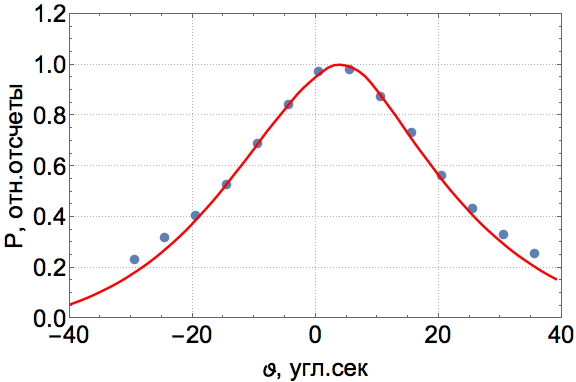
\includegraphics[width=0.45\textwidth]{images/disspers_220_660_300mcm.png}\label{fig:}}
  \caption{Двухкристальная КДО для схемы с кристаллом монохроматором Si(220) - $\theta_B = 10.6^o$ для дисперсионного случая для разных размеров щелевых устройств}
  \label{ris:disspersion_curves_expantheory}
\end{figure}

 В отличие от бездисперсионных КДО (раздел \ref{sec:non_disspers_KDO_section}) заметно присутствует
 влияние размера щелевых устройств.
